\documentclass[DM,authoryear,toc]{lsstdoc}
% lsstdoc documentation: https://lsst-texmf.lsst.io/lsstdoc.html
\input{meta}

% Package imports go here.
\usepackage{physics}
\usepackage{graphicx}
\usepackage{amsmath}
\usepackage{amsfonts}
\usepackage{cleveref}
\usepackage{afterpage}
% Local commands go here.

%If you want glossaries
%\input{aglossary.tex}
%\makeglossaries

\title{The ZOGY image differencing matching kernel and PSF solutions
  and their practical implementation issues}

% Optional subtitle
% \setDocSubtitle{A subtitle}

\author{%
G\'abor Kov\'acs
}

\setDocRef{DMTN-179}
\setDocUpstreamLocation{\url{https://github.com/lsst-dm/dmtn-179}}

\date{\vcsDate}

% Optional: name of the document's curator
% \setDocCurator{The Curator of this Document}

\setDocAbstract{We present the ideal matching kernel and PSF
  solutions for Gaussian input PSFs in the ZOGY image matching, noise
  decorrelation and subtraction method. We discuss sources of
  numerical noise in Fourier-space calculations that can lead to
  spatially badly bound image artifacts in the difference images. We
  briefly study the connection between the Alard-Lupton PSF
  matching with the decorrelation afterburner and the ZOGY
  subtraction methods.}

% Change history defined here.
% Order: oldest first.
% Fields: VERSION, DATE, DESCRIPTION, OWNER NAME.
% See LPM-51 for version number policy.
\setDocChangeRecord{%
  \addtohist{1}{2021-02-01}{Initial release.}{Gabor Kovacs}
  \addtohist{1.1}{2021-03-10}{Fix abstract. Expand the discussion about the decorrelation afterburner.}{Gabor Kovacs}
}

\begin{document}

% Create the title page.
\maketitle
% Frequently for a technote we do not want a title page  uncomment this to remove the title page and changelog.
% use \mkshorttitle to remove the extra pages

% ADD CONTENT HERE
% You can also use the \input command to include several content files.
\section{The derivation of the ZOGY difference image}
%
\par In this document, we study some practical issues of performing
the ZOGY subtraction and its relation to the Alard--Lupton (AL) method
\citep{AL1998} combined with the decorrelation afterburner. We assume
that the reader is somewhat familiar with the Zackay--Ofek--Gal-Yam
(ZOGY) algorithm deduction steps in the ZOGY
paper\citep{ZOGY2016} Appendix A.
%
\par We recall four key ideas behind the ZOGY subtraction method: a) Given
an image with uncorrelated, homoscedastic pixel noise (the noise variance in
each pixel is the same value all over the image), its convolution with an
arbitrary kernel leads to noise correlation between the resulting
pixels. However, in frequency space, the frequencies remain independent (as
random variables), only the amplitude (variance) of their noise content
changes. b) The independent frequency space pixels are complex Gaussian
random variables. For a signal detection purpose, similar log
probability expressions can be written as for the real-valued random
variables (image pixels). c) Log probability can be calculated as a sum over
all the independent frequencies, weighting the squared absolute difference
at each frequency with its inverse noise variance. d) The detection
statistic in frequency space can be split into two multiplicative terms. In
image space, these two terms can be interpreted as a difference image and
its PSF, which produces a per-pixel detection statistic by convolution. The
difference image is constructed in frequency space so that each frequency
bin is a (complex) random variable and has the same variance. This implies
that the difference image in image space has uncorrelated (and under the
model assumptions), homoscedastic noise in its pixels. The difference image
noise remains uncorrelated despite the PSF matching procedure.
%
We recall the following equations from the ZOGY paper.
The new \(N\) science and the reference \(R\) images are modeled as:
\begin{align}
R &= F_rT\otimes P_r + \epsilon_r\\
N &= F_nT\otimes P_n + \epsilon_n
\label{eq:N}
\end{align}
where \(F_r, F_n\) are photometric scaling constants, \(T\) is the
\emph{truth} image, \(P_r, P_n\) are the image PSFs and \(\epsilon_r,
\epsilon_n\) are per-pixel Gaussian white noise with homogenous variance in
the images.
%
\par The detection statistic of \(N\) having a different \(T\) value than \(R\)
at any pixel position can be written in frequency space as:
\begin{equation}
  \hat{S} = \frac{F_nF_r^2\overline{\hat{P}_n}\abs{\hat{P}_r}^2 \hat{N}
 - F_rF_n^2\overline{\hat{P}_r}\abs{\hat{P}_n}^2 \hat{R}
}
{ \sigma_r^2F_n^2\abs{\hat{P}_n}^2 + \sigma_n^2F_r^2\abs{\hat{P}_r}^2 }
\label{eq:S}
\end{equation}
In image space, \(S\) is called the score or significance image and
represents the significance of a source detection for each pixel.
%
The difference image is defined as:
\begin{equation}
\hat{D} = \frac{F_r \hat{P}_r\hat{N} - F_n \hat{P}_n \hat{R}}
{\sqrt{\sigma_r^2F_n^2\abs{\hat{P}_n}^2 + \sigma_n^2F_r^2\abs{\hat{P}_r}^2}}
\label{eq:Dhat}
\end{equation}
and its PSF:
\begin{equation}
\hat{P}_D = \frac{F_rF_n\hat{P}_n\hat{P}_r}
{F_D\sqrt{\sigma_r^2F_n^2\abs{\hat{P}_n}^2 +
    \sigma_n^2F_r^2\abs{\hat{P}_r}^2}}
\label{eq:Pdhat}
\end{equation}
so that:
\begin{equation}
\hat{S} = F_D\hat{D}\overline{\hat{P}_D}
\label{eq:Shat}
\end{equation}
The difference image (and similarly the score image) can be written as the
difference of two ``matched'' images as in \Cref{eq:c1N_c2R}.
\begin{equation}
\hat{D}_z = \frac{\frac{\hat{P}_r}{F_n}}
{\sqrt{\frac{\sigma_n^2}{F_n^2}\abs{\hat{P}_r}^2
 + \frac{\sigma_r^2}{F_r^2}\abs{\hat{P}_n}^2}}
\hat{N} -
\frac{\frac{\hat{P}_n}{F_r}}
{\sqrt{\frac{\sigma_n^2}{F_n^2}\abs{\hat{P}_r}^2
 + \frac{\sigma_r^2}{F_r^2}\abs{\hat{P}_n}^2}}
\hat{R}
=
\hat{c}_n \hat{N} - \hat{c}_r\hat{R}
\label{eq:c1N_c2R}
\end{equation}
%
\par Here \(\hat{c}_n\) and \(\hat{c}_r\) are the matching kernels for
the original science and template images. If the original image PSFs
are accurately described by \(P_r, P_n\), then the frequency space
multiplications transform the PSFs of the two images to be identical,
\(P_D\), \Cref{eq:Pdhat}. Note that while we followed the terminology
of the ZOGY paper here and referred to the images as science and
reference images, the entire ZOGY method is symmetrical to the swapping
of the images. In the following, we may simply denote images with 1
and 2 indices.
%
\section{Discussion points}
We list the following questions that can define the direction of future
ZOGY image differencing code development in the LSST stack.
%
\par How does an ideal Gaussian PSF point source look like theoretically in
a ZOGY difference image? Discussed in \Cref{sec:ZOGYtheo}.  In
\Cref{sec:ZOGYFFT}, we look for answers: What causes the extensive,
oscillating visual patterns in the ZOGY difference image around certain
sources and image features (\Cref{sec:FFTlimits})? What shall we do with the
numerical problems that appear in certain regions in frequency space and
appear as pattern artifacts in image space (\Cref{sec:workaround})? Shall we
implement a Gaussian PSF approximator that produces the PSF frequency space
representation directly?  Shall we implement a Gaussian PSF width estimation
to determine which input PSF is sharper so that a realistic limiting value
can be used at frequencies when both PSFs (in frequency space) are below a
threshold (\Cref{sec:workaround})?  How shall we handle
division by zero scenarios in the ZOGY difference and significance image
calculation (\Cref{sec:PSFzero})?
%
\par In the Appendix, among other smaller topics, we raise the question whether
we can use zero padding for calculating the score image, or shall we use
model white noise padding (\Cref{sec:zeropadS})?
%
\section{The theoretical solution of the ZOGY matching kernel and difference
image PSF\label{sec:ZOGYtheo}}
%
\par In this section, we derive numerical solutions for pure Gaussian
PSFs. The inverse Fourier transforms of the ZOGY matching
kernel or difference image PSF expressions are not expressible in closed
symbolic forms, even in this case. We perform numerical integration of the
functions.
%
\begin{figure}
\begin{center}
  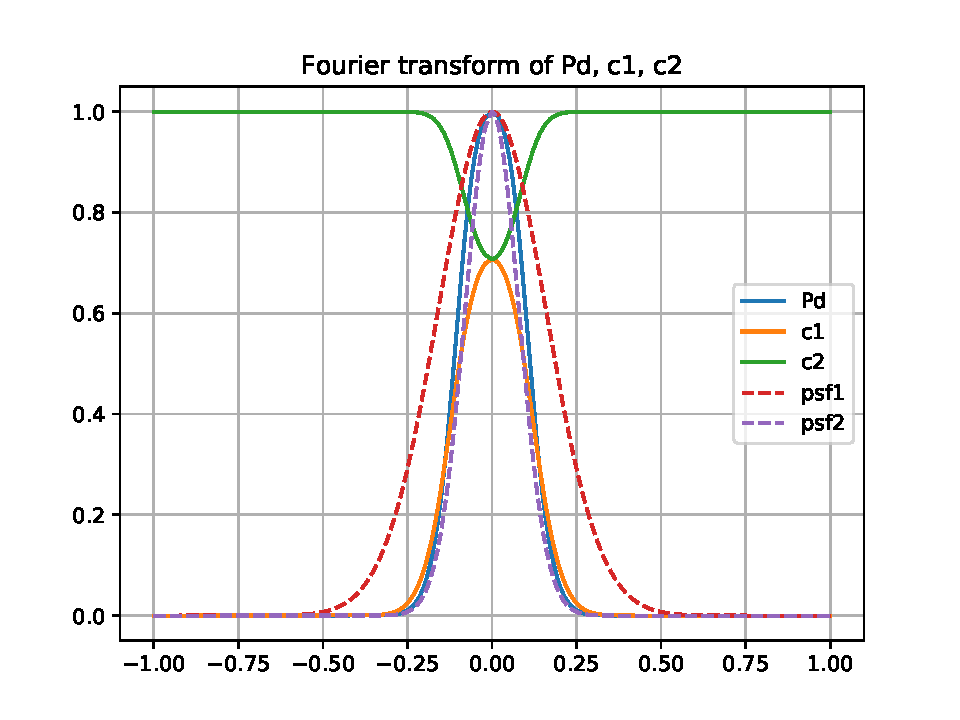
\includegraphics[width=5.5in]{fig/zogy_theo_Gaussians_ft_Pd_c1_c2.pdf}
\end{center}
\caption{\label{fig:theo_Gaussians_ft}1D slice along the x-axis in frequency
  space of the matching kernels and the PSF of the ZOGY difference
  image. The Fourier space representation of the input PSFs is also
  shown. The two PSFs have widths of $\sigma_1 = 1$, $\sigma_2 = 2$ in image
  space, i.e.\ \(\mathrm{PSF}_1\) is originally the narrower but the Fourier
  transformation swaps this relation.}
\end{figure}
%
\par In \Cref{fig:theo_Gaussians_ft}, we show 1D slices of the 2D solutions
of \(P_d\), \(c_1\) and \(c_2\). Noise variances and photometric scaling
factors are unity for simplicity. As the input PSFs are pure Gaussians,
i.e.\ symmetric, real value functions, their Fourier transforms are also
real and symmetric.\footnote{Detailed calculation notebooks are part of
  DM-26087.} Note the different behavior of the two matching kernels towards
high frequencies. The matching kernel of the narrower PSF image \(c_1\) goes
to zero, while the other one goes to unity here. While the graphs of \(c_1\)
and \(c_2\) resemble to Gaussians, they are not anymore, and we must use
numerical integration to calculate their inverse Fourier transform. Their
image space values for points along the x-axis is shown in
\Cref{fig:theo_Gaussians_img_c1,fig:theo_Gaussians_img_c2}.
%
\begin{figure}
\begin{center}
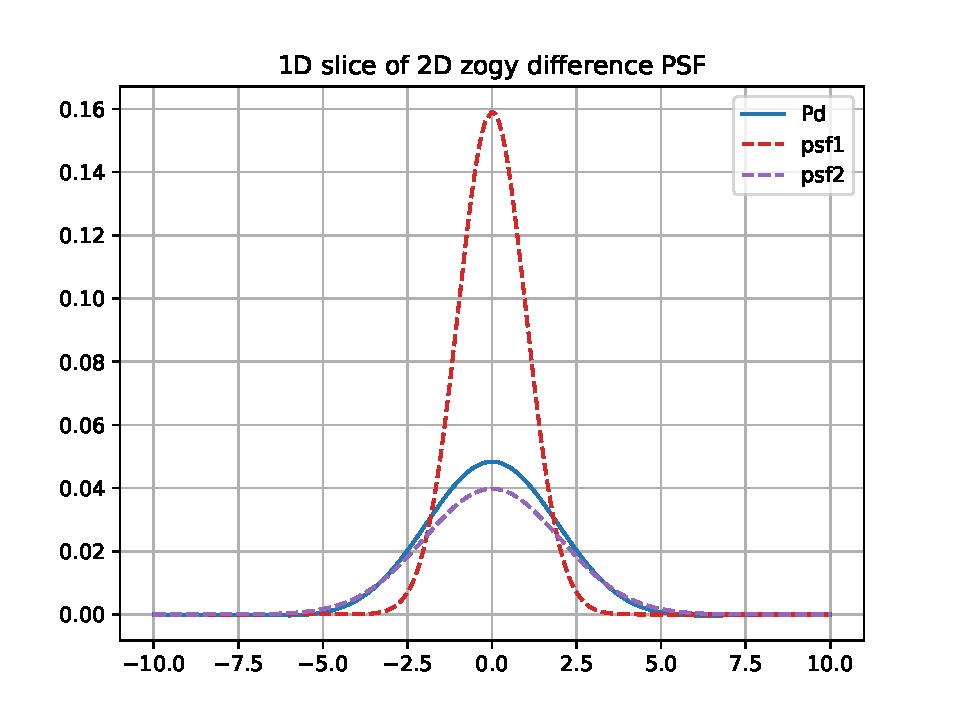
\includegraphics[width=5.5in]{fig/zogy_theo_Gaussians_img_Pd.pdf}
\end{center}
\caption{\label{fig:theo_Gaussians_img_Pd}1D slice along the x-axis in image
  space of the PSF of the ZOGY difference image with the input image PSFs.}
\end{figure}
%
\par In \Cref{fig:theo_Gaussians_img_Pd}, the PSF of the ZOGY difference
  image is shown. It is close to the wider input PSF, but strictly it's not
  a Gaussian, it has a negative overshoot, about 1\% of its peak
  value. This means that in an ideal case, signals in a ZOGY difference
  image are expected to have small negative rings around their positive
  peaks.
%
\begin{figure}
\begin{center}
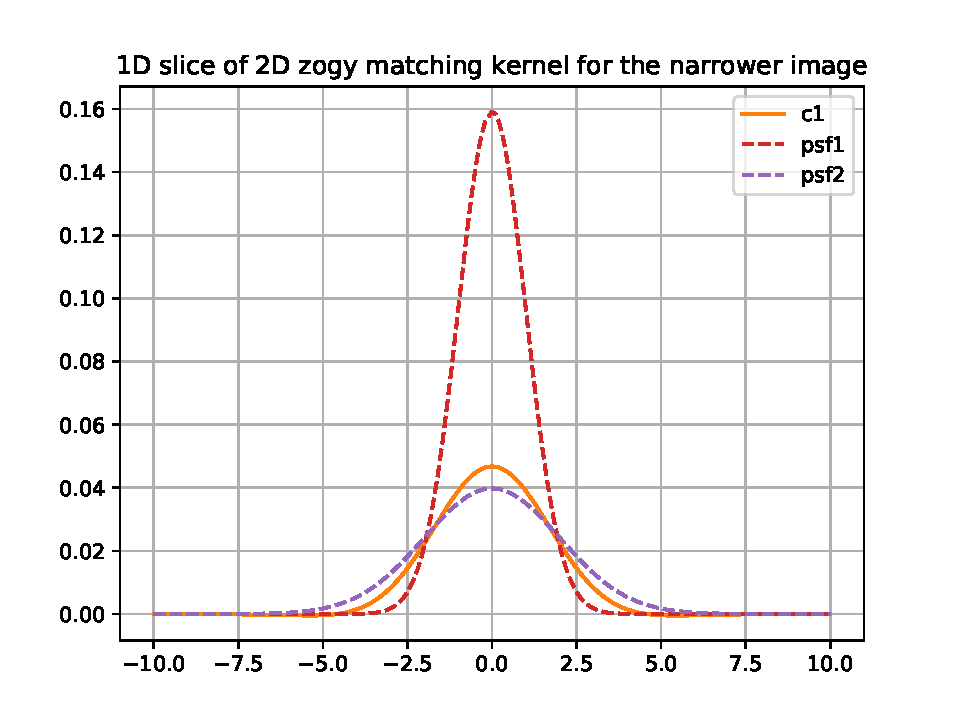
\includegraphics[width=4.5in]{fig/zogy_theo_Gaussians_img_c1.pdf}
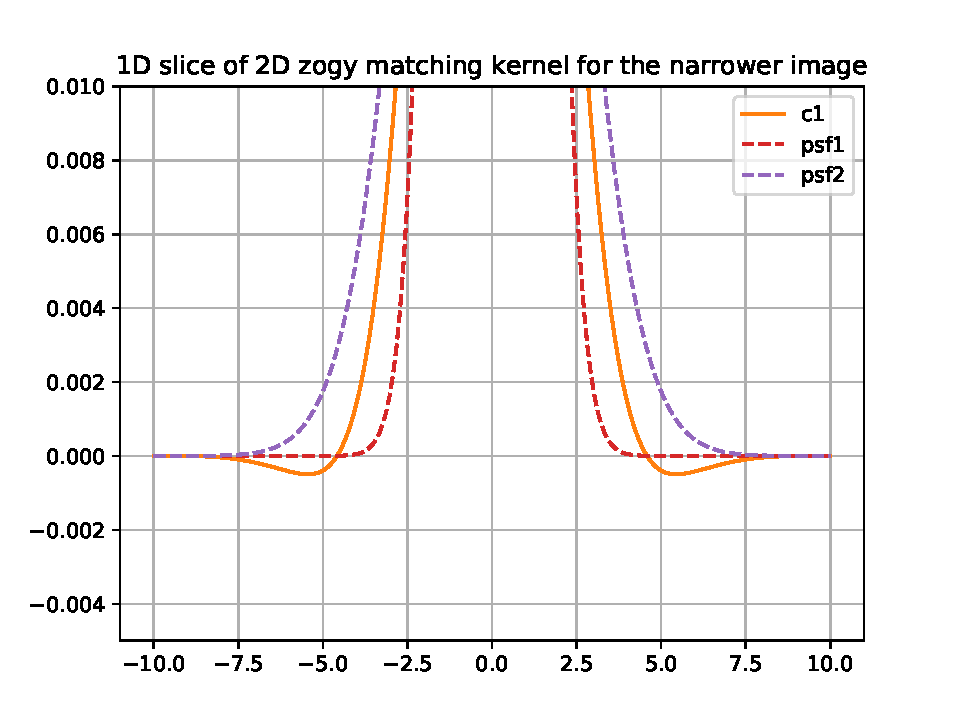
\includegraphics[width=4.5in]{fig/zogy_theo_Gaussians_img_c1_tails.pdf}
\end{center}
\caption{\label{fig:theo_Gaussians_img_c1}1D slice along the x-axis in image
  space of the matching kernel for the narrower PSF image. The matching
  kernel is a Gaussian-like curve that has a small oscillating correction in
  the tails.}
\end{figure}
%
\par For the narrower PSF input image, the matched PSF is created by
convolution with the matching kernel \(c_1\), shown in
\Cref{fig:theo_Gaussians_img_c1}. This matching kernel is similar to usual
Gaussian blurring but slightly narrower and has a negative tail itself.
%
\begin{figure}
\begin{center}
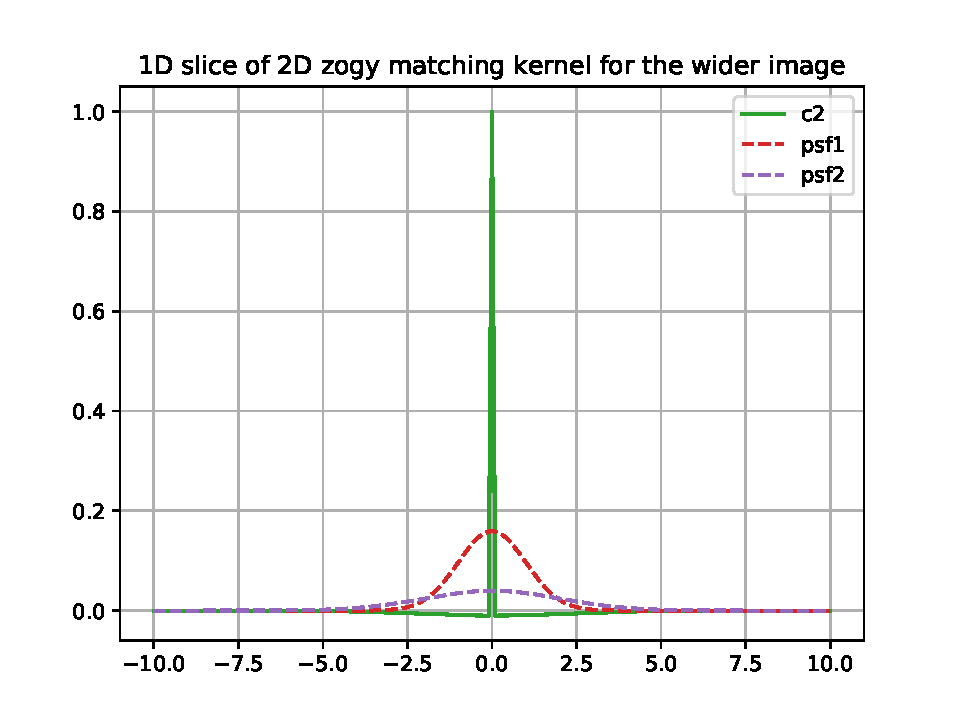
\includegraphics[width=4.5in]{fig/zogy_theo_Gaussians_img_c2.pdf}\,
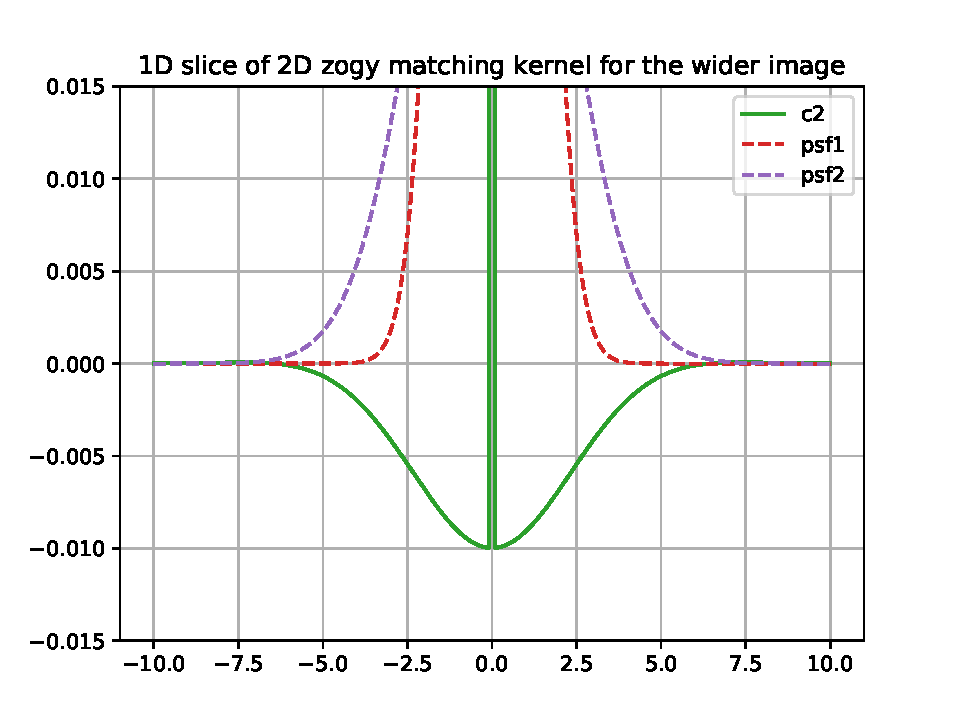
\includegraphics[width=4.5in]{fig/zogy_theo_Gaussians_img_c2_tails.pdf}
\end{center}
\caption{\label{fig:theo_Gaussians_img_c2}1D slice along the x-axis in image
  space of the matching kernel for the wider PSF image. The matching kernel
 is the sum of a Dirac delta minus a Gaussian-like curve.}
\end{figure}
%
\par For the wider image, the matching kernel \(c_2\) is an identity Dirac
delta kernel minus a Gaussian-like correction
(\Cref{fig:theo_Gaussians_img_c2}). The Dirac delta is the inverse transform
of the non-zero constant level of \(c_2\) in \Cref{fig:theo_Gaussians_ft}
that must be subtracted for the numerical integration to converge. The Dirac
delta peak is manually added to the result in \Cref{fig:theo_Gaussians_img_c2}.
%
\par Note that in case of identical PSFs, both \(c_1\) and \(c_2\) become
constant in \Cref{fig:theo_Gaussians_ft} which correspond to Dirac deltas in
image space. I.e. the matching operation is naturally reduced to the
identity operation if the two PSFs are already identical.
%
\clearpage
%
\section{The FFT calculated matching kernel of the ZOGY difference image\label{sec:ZOGYFFT}}
%
\par In practice, the ZOGY subtraction is implemented by Fast Fourier
Transforms (FFT). In this and the following sections, we study
practical numerical aspects of this approach.
%
\par In \Cref{fig:hits_zogy_artifacts}, we show typical patterns that appear
around features that do not subtract well. These sources are present in all
visits in the HiTS2015 data AL image difference processings and in some
visits they produce different artifacts in the AL subtraction as well;
however, AL artifacts are spatially more localized to the source than in the
ZOGY case. The ZOGY patterns can also appear in the vicinity of masked
regions, cosmic rays, or close to the image edges.
%
\begin{figure}
\begin{center}
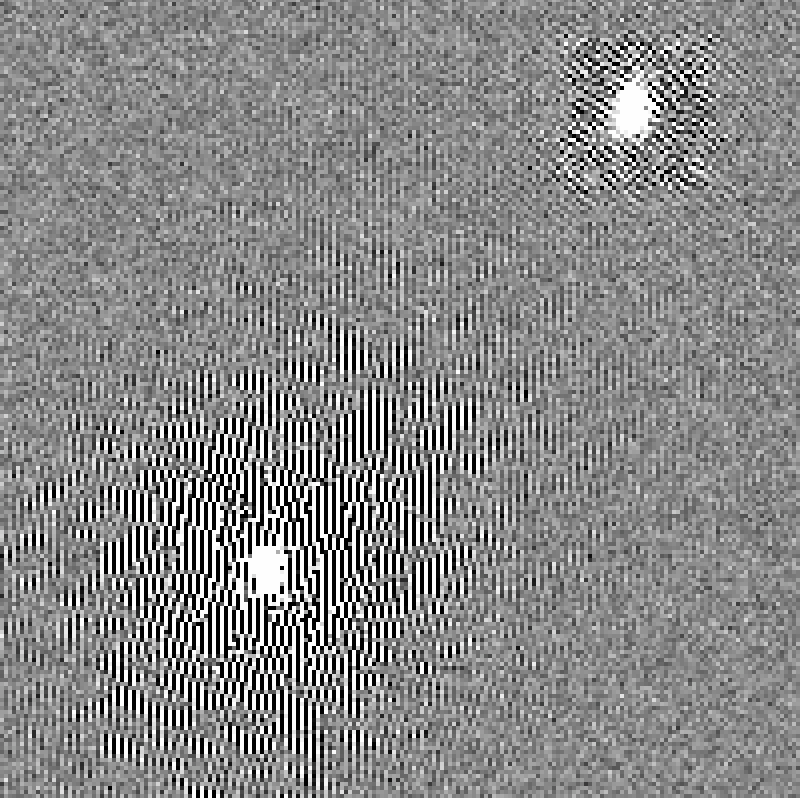
\includegraphics[width=3in]{fig/zogy_artifacts_v412060.png}
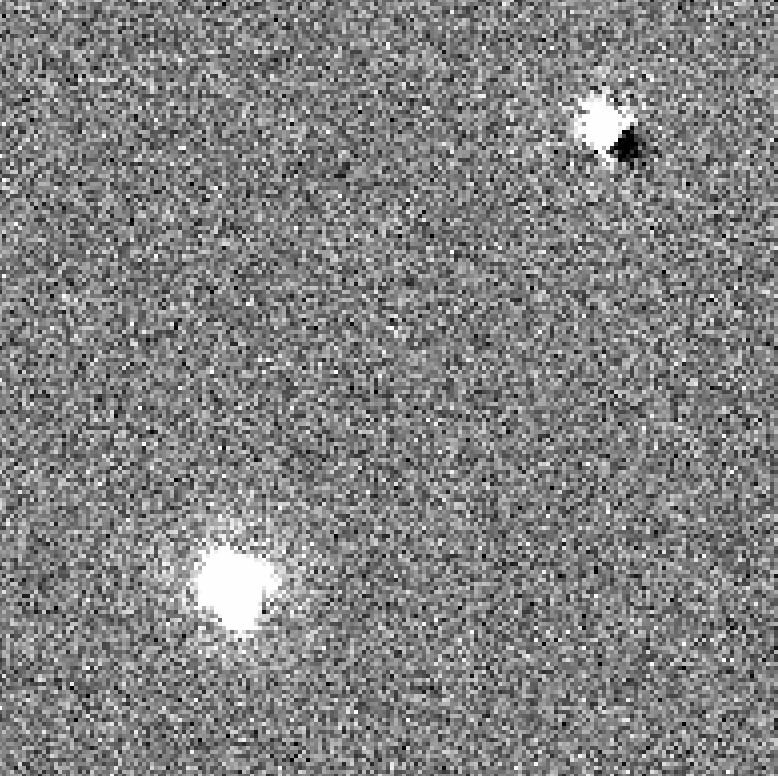
\includegraphics[width=3in]{fig/AL_goodvisit_v412060.png}
\end{center}
\caption{\label{fig:hits_zogy_artifacts}High frequency artifacts in the ZOGY
  difference image (left) around bright sources that are present in all
  visits in the AL processing as well. In the same visit, the AL subtraction
  (right) has less pronounced visual imperfections.}
\end{figure}
%
\subsection{Zero values of the PSF\label{sec:PSFzero}}
%
\par In \Cref{eq:Dhat}, \(\hat{D}\) is not defined at frequencies where both
image PSFs are zero. Indeed, according to the image models (\Cref{eq:N}), at
these frequencies, the input images do not carry any information about the
true image. They consist of pure noise. In accordance with this, these
frequencies have zero contribution to \(\hat{S}\).
%
\par We cannot allow zero division in our calculations anyway, thus we
need to have a workaround for pixels where the denominator in
\Cref{eq:S,eq:Dhat} are zero. We define \(\hat{D}\) at these
frequencies as the straightforward subtraction of the two images with
the same scaling to keep the variance constant at all
frequencies. Of course, \(\hat{S}=0\) at these pixels. This is
currently implemented in the code stack.
%
\subsection{Matching kernel limit values in frequency space\label{sec:FFTlimits}}
\begin{figure}
\begin{center}
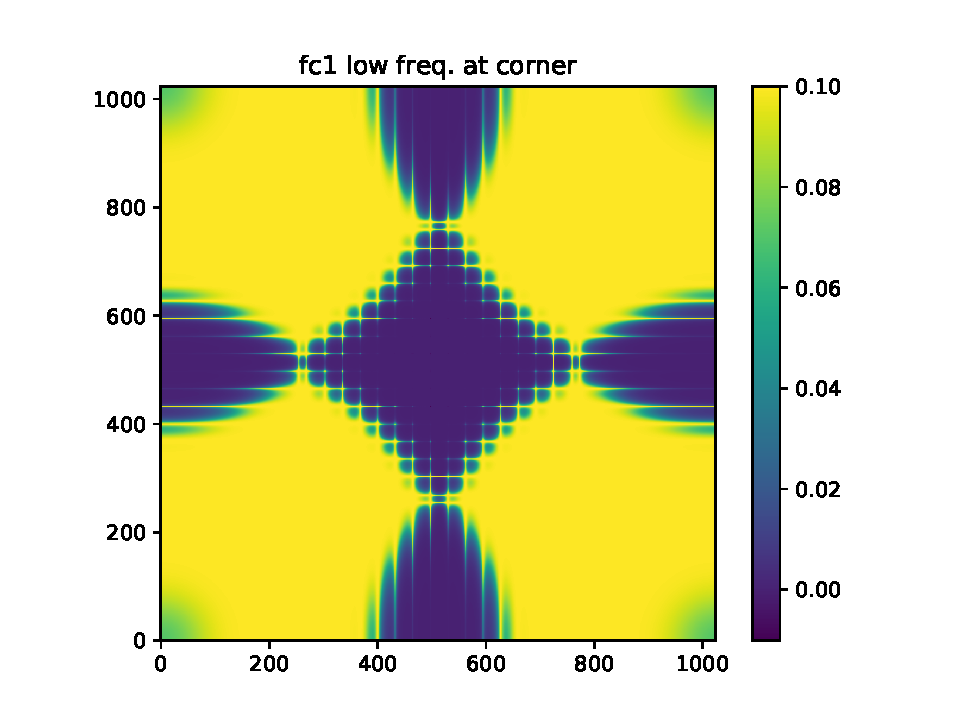
\includegraphics[width=5.5in]{fig/fft_steps_fc1.pdf}
\end{center}
\caption{\label{fig:fft_steps_fc1}FFT calculated matching kernel for two
  Gaussian PSFs, here for the wider PSF image. This is a Fourier space image
  with low frequencies at the corners. In this calculation \(\sigma_1=3.3\),
  \(\sigma_2=2.2\) PSFs were generated in a 31x31 size image, that were zero
  padded to 1024x1024 image size before FFT. Per pixel noise variance is 100
  for both images, photometric scalings are unity. All values are real due
  to symmetry in the inputs.}
\end{figure}
%
\begin{figure}
\begin{center}
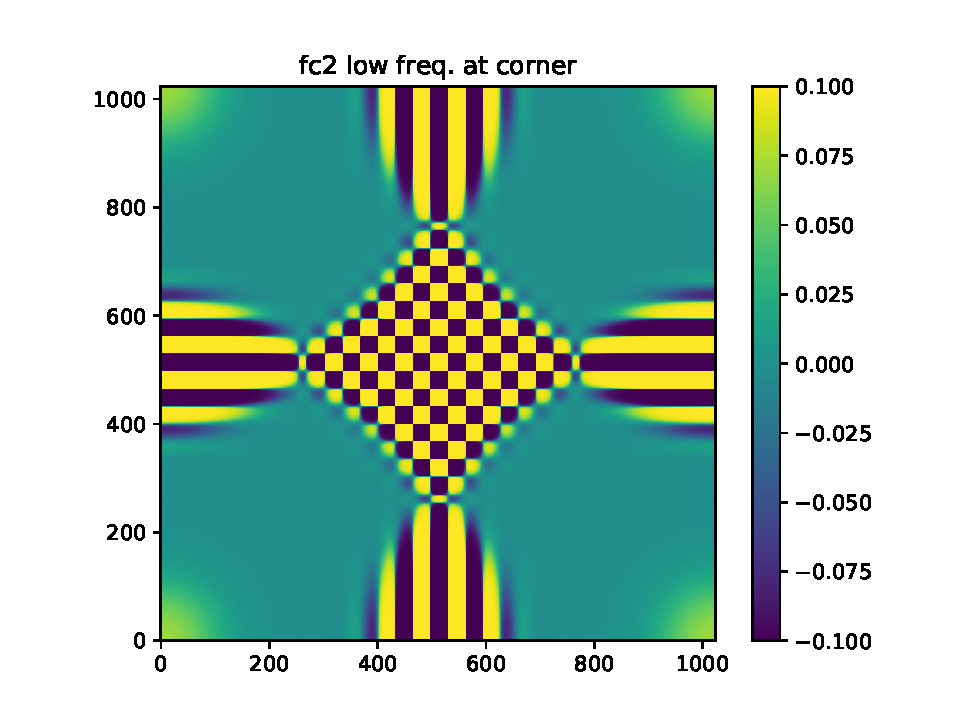
\includegraphics[width=5.5in]{fig/fft_steps_fc2.pdf}
\end{center}
\caption{\label{fig:fft_steps_fc2}FFT calculated matching kernel for the
  narrower PSF image. This is a Fourier space image with low frequencies at
  the corners. All values are real due to symmetry in the inputs.}
\end{figure}
%
\par We saw in the theoretical solution section, that in case of
Gaussian PSF-s, the matching kernels in frequency space have tails
converging to different limit values. The limit values are either zero
or a non-zero constant depending on whether the matching kernel belongs
to the narrower or wider input PSF image, respectively.
%
\par In \Cref{fig:fft_steps_fc1,fig:fft_steps_fc2}, \(\hat{c}_1\),
\(\hat{c}_2\) are calculated from two 31x31 pixel size Gaussian PSFs
that were zero padded for a 1024x1024 image size, with
\(\sigma_1=3.3\), \(\sigma_2=2.2\).\footnote{Detailed calculation
notebooks are part of DM-26941.} All numbers are real in this
case. The shown frequency space images are in their natural FFT
orientation with zero frequencies at the corners and highest
frequencies in the centers. Starting from the corners, both solutions
follow our expectations, converging either down to zero or to their
expected non zero constant (\( 1/\sigma_{\mathrm{pixelnoise}} \) )
plateau. The trend breaks for both kernels in high frequency regions
however, and high value noise appears.
\begin{equation}
\hat{c}_1 \sim \frac{1}{\sqrt{1 + \left(\frac{\hat{P}_1}{\hat{P}_2}\right)^2}}
\label{eq:c1conv}
\end{equation}
\par The matching kernel limit values depend on whether
\(\hat{P}_1/\hat{P}_2\) is converging to zero or diverges as it can be seen
in \Cref{eq:c1conv}. Once we reach the point where the Gaussian tails are
dominated by noises\footnote{See \Cref{sec:floating_point}}, the convergence
properties of these fractions become lost and the calculated matching kernel
values significantly deviate from their expected limit values.
%
\subsection{Patterns in image space\label{sec:patterns}}
\par What does this mean for our calculated matching kernels back in
image space?
%
\par In \Cref{fig:twoG_c1}, we show \(c_1\) transformed and
re-centered back to image space (but still in its fully padded image
size). The purple structure indicates that there is a sign oscillation
pattern all across padded size image.
\begin{figure}
\begin{center}
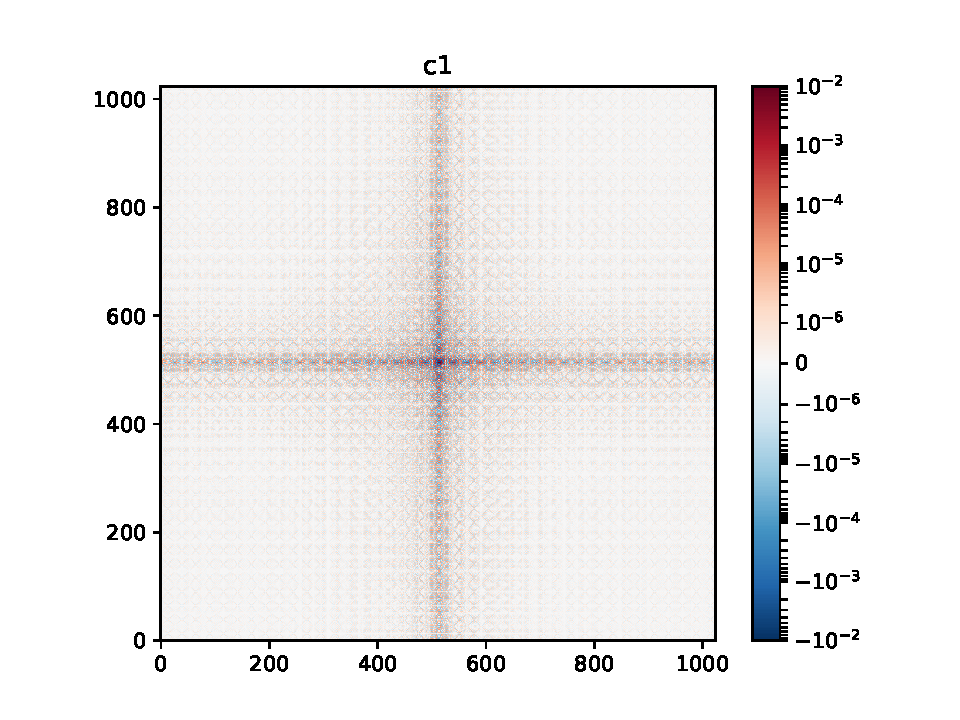
\includegraphics[width=5.5in]{fig/twoG_defaults_c1.pdf}
\end{center}
\caption{\label{fig:twoG_c1}Two Gaussian PSFs with spatial widths of \(\sigma_N = 3.3\)
  \(\sigma_R = 2.2\) pixels. \(c_1\), the ZOGY matching convolution in image space
  of the new (\(N\)) image. The purple pattern is an indication of
  sign oscillation all over the image.}
\end{figure}
%
\par We can see that in the direction of the two axes, there are definite
purplish patterns. The purple color on this red-blue color scale shows a
sign oscillation that can be verified in zoomed-in versions of the
figure. These patterns do not fade away in the direction of the axes from
the center, indicating that these oscillating sign values have roughly the
same order of magnitude absolute values. The original PSF size 31x31 cannot
be clearly identified any more in the image either. We note that
the appearance of these patterns is independent of the padding
size.
%
In \Cref{fig:twoG_pd} \(P_d\) is shown, calculated by \Cref{eq:Pdhat}.
\begin{figure}
\begin{center}
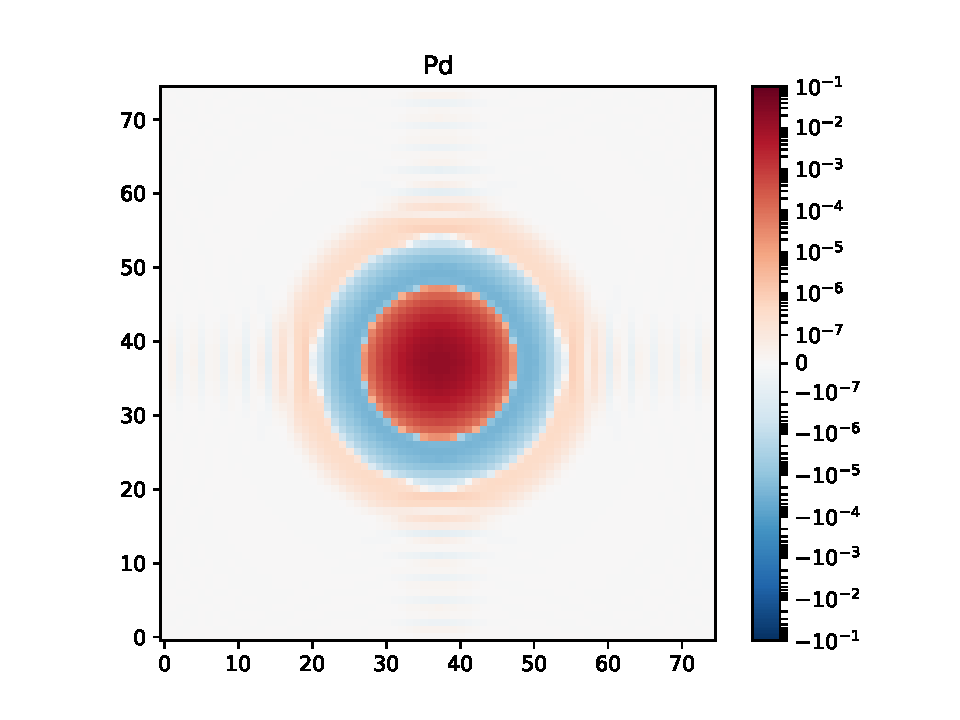
\includegraphics[width=5.5in]{fig/twoG_defaults_Pd.pdf}
\end{center}
\caption{\label{fig:twoG_pd}Two Gaussian PSFs with spatial widths of
  \(\sigma_N = 3.3\) \(\sigma_R = 2.2\). \(P_d\), the PSF of the zogy
  difference image.}
\end{figure}
We also show the PSF of \(S\) in \Cref{fig:twoG_ps}. The PSF of the
score image shows how a Dirac delta signal (in the truth image)
appears in \(S\), though in source detection, only the actual pixel
values matter in \(S\), the shape of the PSF does not.
\begin{figure}
  \begin{center}
    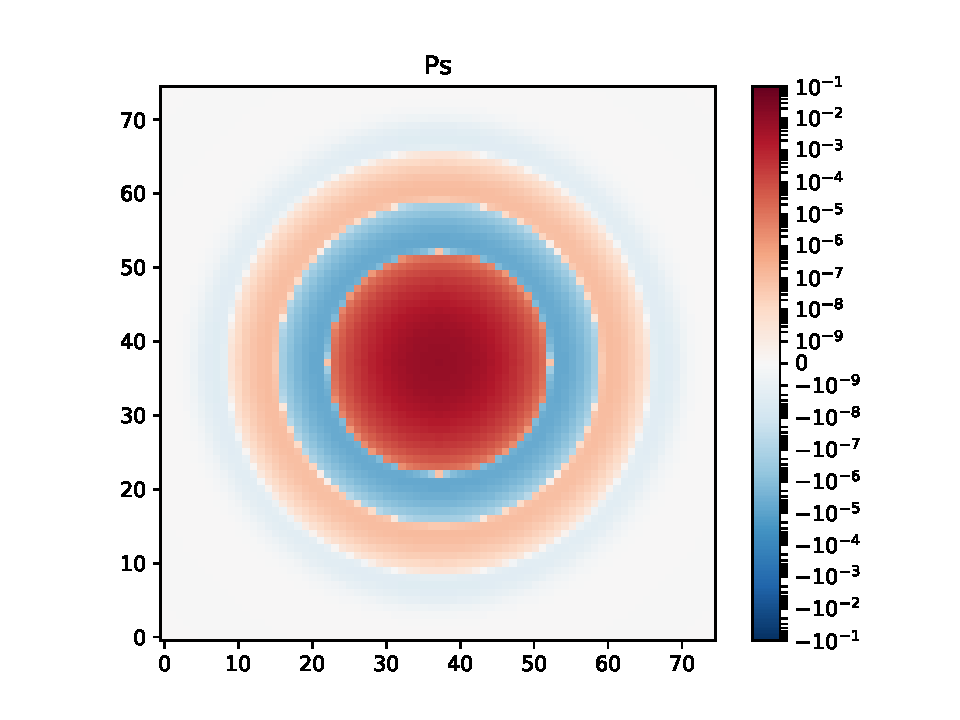
\includegraphics[width=5.5in]{fig/twoG_defaults_Ps.pdf}
  \end{center}
\caption{\label{fig:twoG_ps}Two Gaussian PSFs with spatial widths of
  \(\sigma_N = 3.3\) \(\sigma_R = 2.2\) \(P_s\), the PSF of the score
  image.}
\end{figure}
%
\par \(P_d\) and \(P_s\) have much cleaner images, contained in size
in image space, and close to our theoretical
expectations. (\(\hat{P}_s \sim \hat{P}_d \overline{\hat{P}_d}\)).
%
\par Recall that while we expressed \(P_d\) in \Cref{eq:Pdhat} as the
function of the input PSFs, in a difference image this is the result
of the convolution of the images with the matching kernels.  The high
frequency noise in the matching kernel is not disturbing, so long the
image follows the model PSF assumption and has approximately Gaussian
PSF features that suppress high frequencies. If there are edges, or
signals with high frequency components in the input images, the noisy
high frequency features of the matching kernel becomes visible in the
difference image. Our current understanding is that the deviation of
the image PSF from the model assumption and the numerical noise
in the matching kernels together cause the visible artifacts in the
difference images produced by the code stack. This conclusion is
supported by tests on simulated images that have sources only with
perfect Gaussian PSFs. In these cases, no visual artifacts can be seen.
%
\subsection{Workaround for artifact suppression\label{sec:workaround}}
We propose the following workarounds for the difference image artifact
problem:
\begin{itemize}
  \item In a Gaussian PSF approximation, we can directly create the
    PSF in the padded, full-size frequency space, avoiding the zero
    padding of a small image then the FFT operation. However, this
    approach restricts our input kernels strictly to Gaussians.
  \item In a more generic approach, we can still use the padded, FFT-d
    detected PSFs of the input images. Using a radius approximation, we
    can determine which input PSF is the wider one in a Gaussian
    approximation. Then we can introduce a configurable threshold in
    \emph{frequency space} and pixels in the matching kernels can be
    replaced with their Gaussian limit values wherever the input PSFs
    go below the threshold (in absolute value, in frequency space).
  \item As a third option, we should recall, that the noise artifacts
    appear only in the difference image. In the score image, these are
    automatically suppressed by further convolution with \(P_d\). We
    can choose to use the score image only directly for detection
    significance.
\end{itemize}
%
\par We repeated the above exercise by generating the Gaussian PSFs directly
in frequency space and performed exactly the same matching kernel and
\(P_d\) calculations. These results can be seen in
\Cref{fig:fft_steps_direct_fc1fc2,fig:fft_steps_direct_c1c2,fig:fft_steps_direct_Pd}. These
solutions fully satisfy the theoretical limit values and their image space
counterparts are free from any noisy patterns.
%
\begin{figure}
\begin{center}
  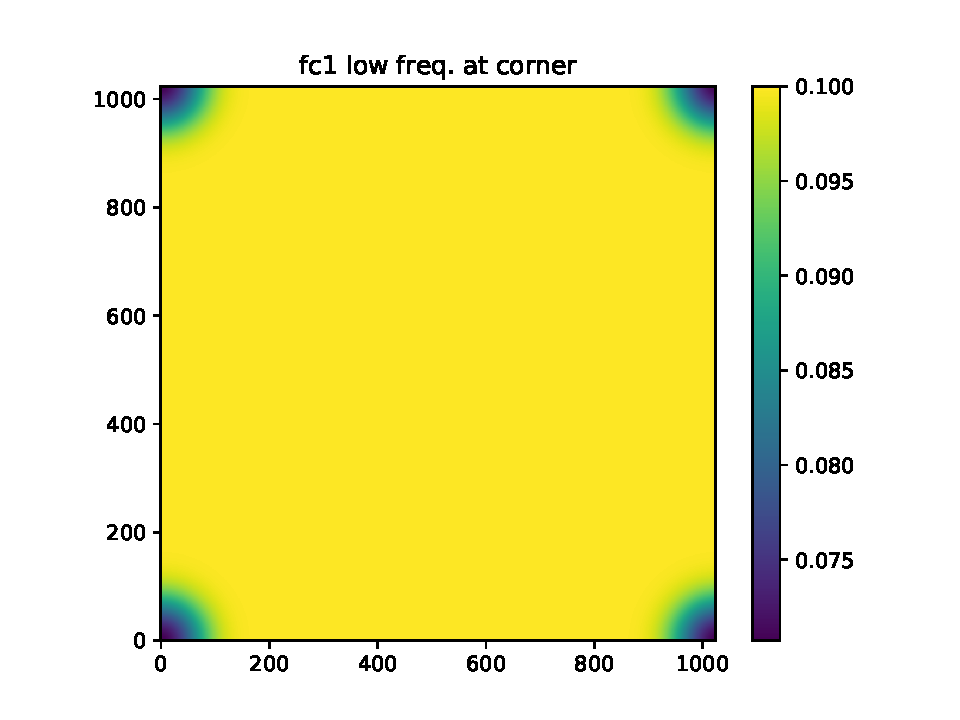
\includegraphics[width=4.5in]{fig/fft_steps_direct_fc1.pdf}
  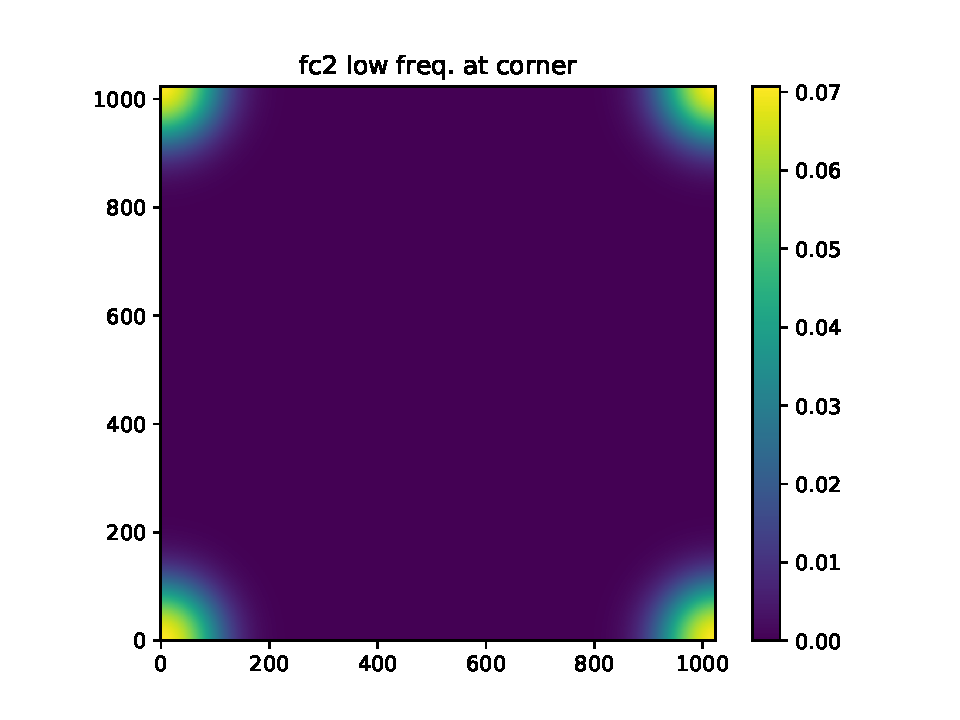
\includegraphics[width=4.5in]{fig/fft_steps_direct_fc2.pdf}
\end{center}
\caption{\label{fig:fft_steps_direct_fc1fc2}The matching kernels for two
  Gaussian PSFs in frequency space. In this calculation, PSFs were
  directly generated in an 1024x1024 frequency space image
  corresponding to image space \(\sigma_1=3.3\), \(\sigma_2=2.2\)
  widths. Per pixel noise variance is 100 for both images, photometric
  scalings are unity.}
\end{figure}
%
\begin{figure}
\begin{center}
  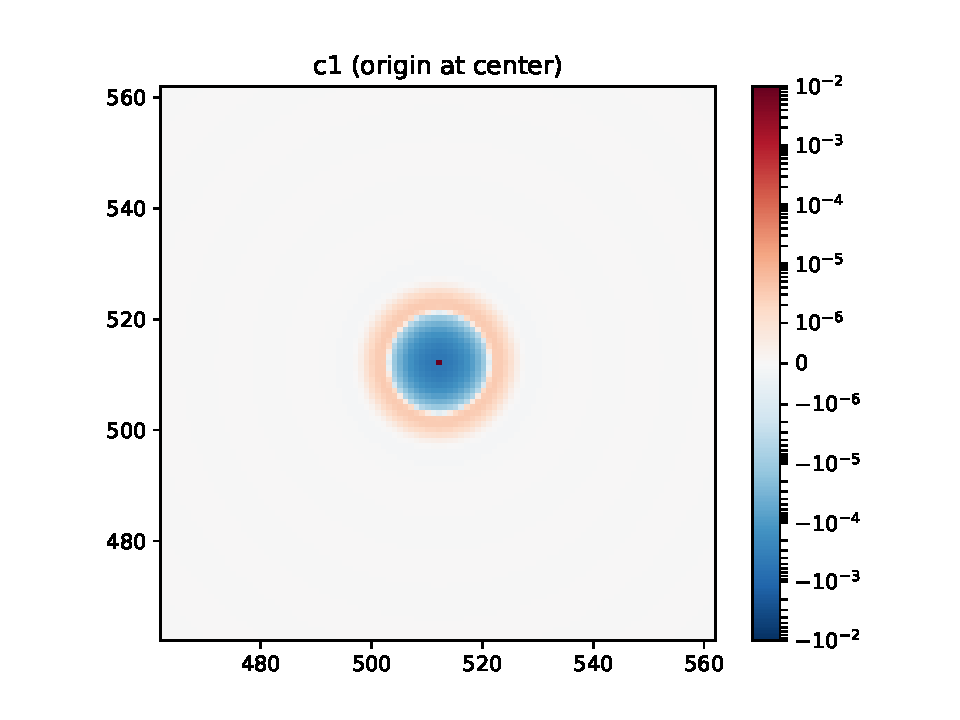
\includegraphics[width=4.5in]{fig/fft_steps_direct_c1_zoomed.pdf}
  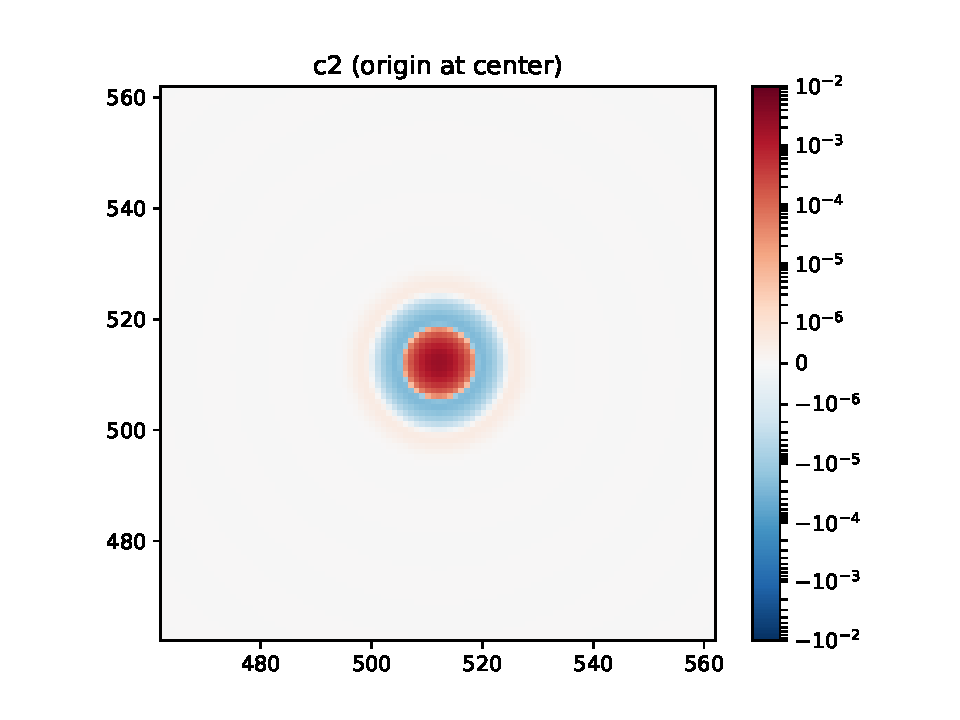
\includegraphics[width=4.5in]{fig/fft_steps_direct_c2_zoomed.pdf}
\end{center}
\caption{\label{fig:fft_steps_direct_c1c2}The matching kernels inverse
  FFT-d into image space, re-centered and zoomed in for
  details.}
\end{figure}
%
\begin{figure}
\begin{center}
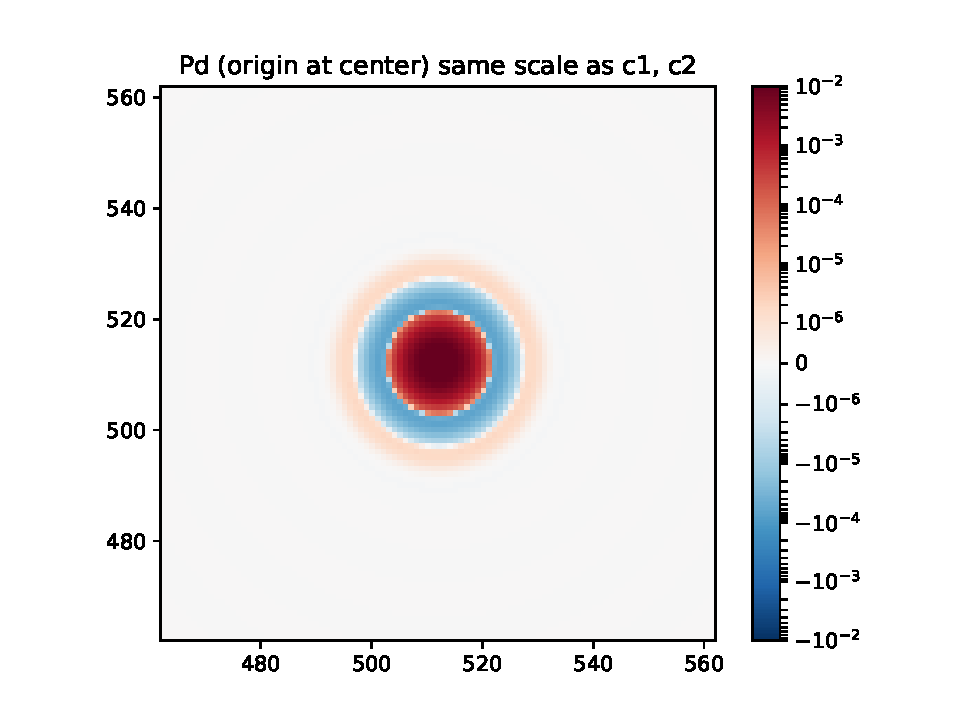
\includegraphics[width=5.5in]{fig/fft_steps_direct_Pd_zoomed.pdf}
\end{center}
\caption{\label{fig:fft_steps_direct_Pd}The difference image PSF
  inverse FFT-d into image space, re-centered and zoomed in for
  details.}
\end{figure}
%
\clearpage
%
\section{Variance plane calculation of the difference image\label{sec:varplane}}
\par While the ZOGY image model does not strictly allow for different
per-pixel noise values (its noise model assumes homogeneous variance
noise across all pixels), from the \Cref{eq:c1N_c2R} form of the
difference image, we can propagate the different pixel variance
information in the variance planes into the difference image. To do
this, we notice that if we do convolution on an image of independent
noise then, in image space, the variance plane should be convolved by
the square of the convolution kernel. This is the well-known square
addition of variances of independent random variables.\footnote{See
  also ZOGY paper eqs. 26-29.}
%
\par We'd like to emphasize that this step cannot be applied to an
image with already correlated noise; the square addition of pixel
noise in the variance plane do not account for the covariance terms
and would result in underestimation of the pixel
variance. Notably, the effect of a noise decorrelation
(whitening) kernel on an already convolved image cannot be applied to
the variance plane based on the square addition rule as it would lower
the variance further instead of reverting it to the uncorrelated
level. In accordance with this, the image space square operation is
not distributive with respect to convolution in general; the square of the
convolution of two kernels is not the same as the convolution of the
squared kernels, and we should always perform the former.
%
\par To calculate the variance plane of the difference image, we
should calculate \(c_n\), \(c_r\) in \Cref{eq:c1N_c2R}, transform them
back to image space, square them in image space, and convolve the
original images' variance planes with these squared matching kernels
(\Cref{eq:VarD}). In practice, this convolution is more
straightforward to be performed in frequency space again because these
images already share common, full image size dimensions (the
dimensions of our ZOGY frequency space calculations).
\begin{align}
  V_D &= V_N \otimes \left(c_n^2\right) + V_R \otimes \left(c_r^2\right)\label{eq:VarD}\\
  \sigma_D^2 &= \sigma_N^2 \sum c_n^2 + \sigma_R^2 \sum c_r^2\label{eq:sigmaD} 
\end{align}
%
\par In the homoscedastic approximation (\Cref{eq:sigmaD}), using the
Parseval theorem (\Cref{sec:parseval}), it can be seen that the zogy
\(\hat{D}\) is scaled (\Cref{eq:Dhat}) so that \(\sigma_D^2 = 1\) for
every pixel, while the flux is scaled to \(F_D\). Note that in the AL
plus decorrelation afterburner case, the flux is preserved, and the
noise variance is scaled to \(\sigma_n^2 / F_n^2 + \sigma_r^2
/F_r^2\). See \Cref{eq:K,eq:KPre}.
%
\par \Cref{eq:Shat} can also be written similarly to \Cref{eq:c1N_c2R}
and the variance plane of S can be calculated analogously
(\Cref{eq:VarD}) this way as well.
%
\section{ZOGY and AL equivalence\label{sec:ALZOGYequiv}}
\par The classic AL algorithm matches the reference image to the new
science image by convolving it with a matching kernel. In frequency
space, the matching kernel solution ideally equals to the quotient of
the two image PSFs as shown in \Cref{eq:Dal}.
%
\begin{equation}
  \hat{D}_{AL} =
  \frac{\hat{P}_{pre}}{F_n}\hat{N} -
    \frac{\hat{P}_{mk}}{F_r}\hat{R}
  =
  \frac{\hat{P}_{pre}\hat{N}}{F_n} -
    \frac{\hat{P}_n\hat{P}_{pre}\hat{R}}{\hat{P}_r F_r}
                 \label{eq:Dal}
\end{equation}
%
\par The decorrelation afterburner was created as a post-processing
correctional step on the difference image. It is calculated in
frequency space so that it decorrelates (whitens) the noise of the
difference image back in image space. We introduce the formula in
\Cref{eq:K} and discuss more details in \Cref{sec:decorrab}.
%
\begin{align}
\hat{K}  &= \frac
  {1}
  {\sqrt{\frac{\sigma_n^2}{F_n^2}\abs{\hat{P}_{pre}}^2 +
      \frac{\sigma_r^2}{F_r^2}\abs{\hat{P}_{mk}}^2}}
  \sqrt{\frac{\sigma_n^2}{F_n^2} + \frac{\sigma_r^2}{F_r^2}}\label{eq:K}
\end{align}
%
\par In \Cref{eq:DzPz,eq:DzPrPrPz,eq:DaldPald}, we write the ZOGY score image in frequency
space and expand the expression to demonstrate that the AL matching
and subtraction combined with the decorrelation afterburner noise
whitening theoretically leads to the same detection statistics.
%
\begin{align}
  \hat{S} \sim \hat{D}_Z\overline{\hat{P}_Z} &= \frac
  {\frac{\hat{P}_r\hat{N}}{F_n} - \frac{\hat{P}_n\hat{R}}{F_r}}
  {\sqrt{\frac{\sigma_n^2}{F_n^2}\abs{\hat{P}_r}^2 +
      \frac{\sigma_r^2}{F_r^2}\abs{\hat{P}_n}^2}}
  \cdot
  \frac{\overline{\hat{P}_n\hat{P}_r}\sqrt{\frac{\sigma_n^2}{F_n^2} + \frac{\sigma_r^2}{F_r^2}}}
  {\sqrt{\frac{\sigma_n^2}{F_n^2}\abs{\hat{P}_r}^2 +
      \frac{\sigma_r^2}{F_r^2}\abs{\hat{P}_n}^2}} = \label{eq:DzPz}\\
 &= F_D \frac
  {\left(\frac{\hat{N}}{F_n} -  \frac{\hat{R}}{F_r} \cdot
    \frac{\hat{P}_n}{\hat{P}_r}\right) \sqrt{\frac{\sigma_n^2}{F_n^2} + \frac{\sigma_r^2}{F_r^2}} }
  {\sqrt{\frac{\sigma_n^2}{F_n^2} +
      \frac{\sigma_r^2}{F_r^2}\abs{\frac{\hat{P}_n}{\hat{P}_r}}^2}}
  \cdot
  \underbrace{
  \frac{\hat{P}_r}{\abs{\hat{P}_r}}
  \cdot
  \frac{\overline{\hat{P}_r}}{\abs{\hat{P}_r}}
  }_{1} % underbrace
  \cdot
  \frac{\overline{\hat{P}_n}\sqrt{\frac{\sigma_n^2}{F_n^2} + \frac{\sigma_r^2}{F_r^2}}}
  {\sqrt{\frac{\sigma_n^2}{F_n^2} +
      \frac{\sigma_r^2}{F_r^2}\frac{\abs{\hat{P}_n}^2}{\abs{\hat{P}_r}^2}}} = \label{eq:DzPrPrPz}\\
  &= F_D \hat{D}_{AL+d} \cdot \frac{\overline{\hat{P}_n}
  \sqrt{\frac{\sigma_n^2}{F_n^2} + \frac{\sigma_r^2}{F_r^2}}}
  {\sqrt{\frac{\sigma_n^2}{F_n^2} +
      \frac{\sigma_r^2}{F_r^2}\abs{\frac{\hat{P}_n}{\hat{P}_r}}^2}} =
F_D \hat{D}_{AL+d}\overline{\hat{P}_{AL+d}}\label{eq:DaldPald}
\end{align}
%
%
\begin{align}
F_D &= \frac{1}{\sqrt{\frac{\sigma_n^2}{F_n^2} +
    \frac{\sigma_r^2}{F_r^2}}} \\
\hat{D}_{AL+d} &= \frac{\hat{D}_Z}{F_D}\cdot\frac{\abs{\hat{P}_r}}{\hat{P}_r}\label{eq:Dald}
\end{align}
%
\par We start with the ZOGY score image in \Cref{eq:DzPz} and
demonstrate that the expression is equivalent with the score
calculated from a perfectly matching, decorrelated AL solution in
\Cref{eq:DaldPald}.  In the AL approach the role of the two images are
not symmetric, the template PSF is matched to the science image, and
the science image is left intact. Assuming that the AL optimization
finds the perfect matching kernel, it should be
\(\hat{P}_n/\hat{P}_r\). Indeed, considering the score image, the
difference between the AL and ZOGY images are only a factor of
\(\hat{P}_r/\abs{\hat{P}_r}\). Compared to the AL, in the ZOGY case
both the difference image and its PSF carry an extra
\(\hat{P}_{r}/\abs{\hat{P}_{r}}\) factor that cancel from the overall
expression of the score image. Indeed, as
\(\overline{\hat{P}_r}\hat{P}_r/\abs{\hat{P}_r}^2 = 1\) at all
frequencies, we can reduce or expand this factor in the difference
image and its PSF terms without changing their resulting product, the
score image.
%
\par Furthermore, note that \(\hat{P}_r/\abs{\hat{P}_r}=1\) itself, if
\(\hat{P}_r\) is real and positive at all frequencies. This is the
case if \(\hat{P}_r\) is a Gaussian PSF function. In this case \(D_Z\)
and \(D_{AL+d}\) are mathematically the same as shown in
\Cref{eq:Dald}; expanding or reducing the fractions in frequency space
by arbitrary real, positive kernels have the corresponding operations
of pre-convolution and deconvolution in image space.
%
\par In the decorrelated AL approach, we can also apply an arbitrary
Gaussian pre-convolution kernel without changing the difference image
in theory. However, calculating \Cref{eq:DalPre} in two separate
steps, as a difference image that is decorrelated afterwards in a
second step is numerically problematic as discussed in
\Cref{sec:decorrab}.
%
\begin{align}
  \hat{D}_{AL+d} =  \hat{D}_{AL} \cdot \hat{K}  &= \frac
  {\frac{\hat{P}_{pre}\hat{N}}{F_n} -
    \frac{\hat{P}_n\hat{P}_{pre}\hat{R}}{\hat{P}_r F_r} }
  {\sqrt{\frac{\sigma_n^2}{F_n^2}\abs{\hat{P}_{pre}}^2 +
      \frac{\sigma_r^2}{F_r^2}\abs{\frac{\hat{P}_n\hat{P}_{pre}}{\hat{P}_r}}^2}}
  \sqrt{\frac{\sigma_n^2}{F_n^2} + \frac{\sigma_r^2}{F_r^2}}
  \label{eq:DalPre}\\
%
  &= \frac
  {\frac{\hat{P}_{pre}}{F_n}\hat{N} -
    \frac{\hat{P}_{mk}}{F_r}\hat{R} }
  {\sqrt{\frac{\sigma_n^2}{F_n^2}\abs{\hat{P}_{pre}}^2 +
      \frac{\sigma_r^2}{F_r^2}\abs{\hat{P}_{mk}}^2}}
  \sqrt{\frac{\sigma_n^2}{F_n^2} + \frac{\sigma_r^2}{F_r^2}}\label{eq:DaldPreMk}
\end{align}
%
\section{The decorrelation afterburner\label{sec:decorrab}}
Let's consider the decorrelation afterburner first without the
pre-convolution kernel, when (\(\hat{P}_{pre}=1\)) at all frequencies
in \Cref{eq:K}.
%
\par Assuming a Gaussian matching kernel (\(\hat{P}_{mk}\)) that
converges to zero towards high frequencies, the overall expression of
\(\hat{K}\) in \Cref{eq:K} converges to \(F_{n}/\sigma_n\). The
decorrelation correction function in frequency space is similar to
\(\hat{c}_2\) in \Cref{fig:theo_Gaussians_ft}. In image space, its
graph follows a dirac delta plus a negative overshoot as in
\Cref{fig:theo_Gaussians_img_c2}. In the straightforward AL case, when
we convolve the template image, we don't expect any complication in
calculating such a decorrelation correction. As \(\sigma_r \ll
\sigma_n\), \Cref{eq:K} can keep its convergence properties even if
\(\hat{P}_{mk}\) values are noisy in their Gaussian tails.
%
\par Now let's consider the swapped image case, when we convolve the
science image.  The numerical stability of this case is less
certain. As \(\sigma_r \gg \sigma_n\) in this case, it can prevent
\(\sigma_{n}^2/F_n^2\) from becoming the dominant term in the
denominator of \Cref{eq:K} and the numerical noise in the tails of
\(\hat{P}_{mk}\) may remain in the high frequency values \(\hat{K}\).
%
\par Let's assume now a Gaussian pre-convolution kernel. It can be
seen that the overall expression of \(\hat{K}\) becomes divergent in
\Cref{eq:K} towards high frequencies. The denominator converges to
zero. Even if we don't directly hit numerical overflows in calculating
\(\hat{K}\), a divergent \(\hat{K}\) cannot be meaningfully
applied. The difference image converges to zero (\(\hat{D}_{AL}\),
\Cref{eq:Dal}), so correcting the already computed difference image is
similar to inverting a multiplication operation of smaller and smaller
numbers. In \Cref{eq:DaldPreMk}, we can see that calculating the
corrected difference image (\(\hat{D}_{AL+d}\)) is exactly the same
problem as calculating the ZOGY difference image in \Cref{eq:Dhat}. In
these expressions, both the numerators and the denominators converge to
zero which in practice result in numerical noise in the tail regions
of the input Gaussians (image PSFs, pre-convolution and matching
kernels). We face the very same numerical problems that was discussed
in \Cref{sec:ZOGYFFT}.
% 
\subsection{Decorrelation afterburner with pre-convolution\label{sec:decorr_preconv}}
%
\par We saw that the decorrelation afterburner of \Cref{eq:K} is
problematic if we use a pre-convolution kernel. In this form the
decorrelation afterburner wants to recover the proper difference
image, inverting the pre-convolution operation completely.
%
\par Recall that pre-convolution is a practical way to ensure that the
science image PSF is wider than our template PSF. We also know that if
we choose to correlate an image with its own
PSF\footnote{Pre-convolution with the flipped PSF in image space;
  multiplication with complex conjugate in frequency space (e.g.\
  \Cref{eq:Shat}).}, under the independent Gaussian noise model
assumptions, we get a detection likelihood image.
%
\par We show here that we can apply a form of the decorrelation
afterburner in the pre-convolution case if we pre-convolve the science
image with its own PSF. This form of the decorrelation afterburner
does not invert the pre-convolution operation, in this sense it does
not do noise decorrelation any more. Rather it corrects the
pre-convoled and AL PSF matched likelhood difference image directly
and results in the equivalent of the zogy score image as an optimal
detection statistics in the case when both the science and template
images have noise.
%
We can rewrite \Cref{eq:S}:
\begin{align}
  \hat{S} &= 
            \frac{\overline{\hat{P}_n} \frac{\hat{N}}{F_n} -
            \frac{\abs{\hat{P}_n}^2}{\hat{P}_r} \frac{\hat{R}}{F_r} }
            % denom
            { \frac{\sigma_n^2}{F_n^2} +
            \frac{\sigma_r^2}{F_r^2}
            \frac{\frac{\abs{\hat{P_n}}^2}{\hat{P}_r}}
            {\overline{\hat{P}_r}}         
            } =
            \frac{\overline{\hat{P}_n} \frac{\hat{N}}{F_n} -
            \frac{\abs{\hat{P}_n}^2}{\hat{P}_r} \frac{\hat{R}}{F_r} }
            % denom
            { \frac{\sigma_n^2}{F_n^2} +
            \frac{\sigma_r^2}{F_r^2}
            \frac{\abs{\hat{P}_{mk}}^2}{\abs{\hat{P}_{n}}^2}
            } = 
            % two terms
            \underbrace{\left(
            \overline{\hat{P}_n} \frac{\hat{N}}{F_n} -
            \frac{\abs{\hat{P}_n}^2}{\hat{P}_r} \frac{\hat{R}}{F_r}
            \right)}_{\textrm{pre-convolved AL}} \cdot
            % denom
            \frac{1}
            { \frac{\sigma_n^2}{F_n^2} +
            \frac{\sigma_r^2}{F_r^2}
            \frac{\abs{\hat{P}_{mk}}^2}{\abs{\hat{P}_{n}}^2}
            }
            \label{eq:SPre}\\
  \hat{P}_{mk} &= \frac{\abs{\hat{P_n}}^2}{\hat{P}_r} \label{eq:Smk}\\
  \hat{S} &= \hat{c}_{sn} \hat{N} - \hat{c}_{sr}\hat{R} =
            \frac{\frac{\overline{\hat{P}_n}}{ F_n} }
            % denom
            { \frac{\sigma_n^2}{F_n^2} +
            \frac{\sigma_r^2}{F_r^2}
            \frac{\abs{\hat{P}_{mk}}^2}{\abs{\hat{P}_{n}}^2}
            } \hat{N}
            -
            \frac{
            \frac{\abs{\hat{P}_n}^2}{\hat{P}_rF_r} }
            % denom
            { \frac{\sigma_n^2}{F_n^2} +
            \frac{\sigma_r^2}{F_r^2}
            \frac{\abs{\hat{P}_{mk}}^2}{\abs{\hat{P}_{n}}^2}
            } \hat{R}\label{eq:Scncr}
\end{align}
%
\par In \Cref{eq:SPre}, the first term in the numerator is the PSF
pre-convolved science image that now has a PSF of
\(\abs{\hat{P}_n}^2\), and the theoretical PSF matching kernel is
written in \Cref{eq:Smk}. We use the matching kernel to express the
correction in \Cref{eq:SPre} on the right side. Compared to the
original decorrelation afterburner expression, the correction is
squared and the correction with the matching kernel is deconvolved
with the pre-convolution kernel.
%
\par Let's consider the convergence properties towards high
frequencies in case of Gaussian PSFs. The numerator of this expression
always goes to zero while the denominator never goes to zero,
irrespectively of the widths of \(\hat{P}_{mk}\) and
\(\hat{P}_{n}\). As such, \(\hat{S}\) always goes to zero.
%
\par If we use pre-convolution to avoid the AL deconvolution case, it
is guaranteed that the matching kernel solution will be narrower in
image space than the PSF of the science image. In frequency space, the
relation is the opposite, and the denominator of \Cref{eq:SPre} should
actually diverge, making the overall zero convergence faster.
%
\par Note that the zero convergence property of \(\hat{S}\) is kept
even if the convergence properties are numerically lost in the second
term of the denominator at high frequencies. Therefore we do not
expect \emph{worse} high frequency noise to appear in our ``afterburned''
likelihood/score image result than it would be in a simple frequency
space PSF convolution operation.
%
\par We emphasize that while we can apply this correction on the
already calculated pre-convolved AL likelihood difference image, we
cannot do it on its variance plane. Because the noise in the score
image is not white, we cannot easily estimate the noise level even in
the homoscedastic noise model case. Instead, we need to follow the
considerations of \Cref{sec:varplane} for the variance plane
calculation and express \(\hat{S}\) with the overall coefficients of
\(\hat{N}\) and \(\hat{R}\) as shown in \Cref{eq:Scncr}. Recall, we
transform \(\hat{c}_{sn}\) and \(\hat{c}_{sr}\) back to image space,
square them in image space, and convolve the original images' variance
planes with these squared matching kernels (\Cref{eq:VarD}). In the
homoscedastic approximation, we multiply \(\sigma_n^2\) and
\(\sigma_r^2\) with the sum of squares (\Cref{eq:sigmaD}), but we
still need to calculate \(c_{sn}\) and \(c_{sr}\). In this
approximation, the inverse FFT of \(\hat{c}_{sn}\) and
\(\hat{c}_{sr}\) can be spared and the sum can be calculated directly
in frequency space (Parseval theorem, \Cref{sec:parseval}).
%
\subsection{Decorrelation afterburner normalization}
\par The classic AL method can be applied to images without
considering their photometric scaling factors (\(F_n, F_r\)). In this
case, the AL optimisation itself solves for the ratio of the
photometric scaling between the images. This scaling appears as the
sum of the AL matching kernel. So far, we've assumed that our AL
matching kernels are normalized like image PSFs. Let's relax this
assumption and separate the sum of the pre-convolution and matching
kernels into standalone factors \(S_{pre}\), \(S_{mk}\). To preserve
the photometric flux, the decorrelation afterburner correction should
still be overall a convolution with a normalized correction kernel in
image space.
%
\par Image space sum normalization can be easily ensured in the
corresponding frequency space expression. If we evaluate any
convolution kernel at 0 frequency, based on \Cref{eq:X0sum} they
should be equal to 1. We should include \(S_{pre}\), \(S_{mk}\) in the
numerator scaling factor to satisfy the normalization criterion. The
normalized decorrelation afterburner can be written as \Cref{eq:KPre}.
%
\begin{align}
  \hat{K} &= \frac{\sqrt{\frac{\sigma_n^2}{F_n^2}S_{pre}^2 + \frac{\sigma_r^2}{F_r^2}S_{mk}^2}}
  {\sqrt{\frac{\sigma_n^2}{F_n^2}S_{pre}^2\abs{\hat{P}_{pre}}^2 + \frac{\sigma_r^2}{F_r^2}S_{mk}^2
  \abs{\hat{P}_{mk}}^2}}
\label{eq:KPre}
\end{align}
%
\par Similarly, should the PSFs be not normalized to sum 1 in the ZOGY
image differencing, the sum of the PSFs should appear in \(F_{D}\) in
the same way as a scaling factor.
%
\subsection{A possible fusion of AL and ZOGY}
To keep the advantage of AL of not assuming a prior knowledge of the
image PSFs and of ZOGY to produce a proper difference image, we
propose the following algorithmic fusion of the two approaches.
%
\par Let's choose a Gaussian pre-convolution kernel (\(P_{pre}\)), so
that the AL algorithm can determine an accurate \(P_{mk}\) reliably in
image space; perhaps in a spatially varying manner for the whole
image. The optimisation of the pre-convolution kernel can focus solely
on the quality of the AL matching kernel solution. The expected
tradeoff here is that the wider the pre-convolution kernel, the easier
to find a Gaussian matching kernel but on the other hand, a wider
pre-convolution kernel means more noise correlation and a less accurate
minimisation in the AL algorithm. We do not need to calculate the
classic AL difference image in its original \Cref{eq:Dal} form here.
%
\par In the next step, using \Cref{eq:DaldPreMk}, we perform a ZOGY
difference image calculation using the \(\hat{P}_{pre}\) and
\(\hat{P}_{mk}\) solutions from the previous step. They behave like
the ``image PSFs'' in the original zogy calculations. We should also
apply all the precautions and numerical considerations discussed
earlier. As \(\hat{P}_{pre}\) is positive and real, it should
disappear completely from the proper difference image and score image
values. We note however, that the wider is \({P}_{pre}\) in image
space, the narrower \(\hat{P}_{pre}\) becomes in frequency
space. While multiplication with a Gaussian functions is fully
invertible theoretically, numerically such a multiplication will
suppress high frequency values and indirectly throws away high
frequency (spatial) information from the score image. This is
different from the tails (and zero points) of the image PSFs. At the
PSF zero points the images do not carry any information, while with
the pre-convolution, we throw away information from the data. Ad
absurdum, imagine that we keep only the 0th frequency in frequency
space. It'd correspond to a pre-convolution kernel of uniform values
in image space. We'd average out our whole images and would get one
uniform detection score for all pixels.
%
\section{Conclusions}
%
\par We studied the ZOGY difference image matching kernels for Gaussian
input PSFs in this document. In the theoretical calculations
(\Cref{sec:ZOGYtheo}), we showed that the matching kernels have different
convergence values in their tails depending whether they belong to the
narrower of wider PSF input image. In practice, using FFT, these convergence
properties are not well reproduced and the resulting image space matching
kernels have oscillating patterns all over the image
(\Cref{sec:ZOGYFFT}). We concluded that this noise is still acceptable if
the input images follow their PSF models and suppress high frequencies,
however noise patterns appear in the difference image if the PSFs
deviate. This noise is extended, visually unappealing, and can disrupt other
algorithms' performance on the difference image; however, it has little
impact on the source detection statistic.
%
\par We tested the direct Gaussian PSF generation in frequency space as a
possible way to avoid the convergence problems in our calculations. We
expect that it would produce difference images without large scale patterns
for all inputs. It is a strong restriction on the PSFs, so we also plan to
look for weaker constraints in suppressing the artifacts in the difference
image. We also need to consider sampling (aliasing) details before
implementation.
%
\par In \Cref{sec:varplane} we discussed how to properly calculate the variance
plane in frequency space when we have noise whitening decorrelation
operations.
%
\par In \Cref{sec:ALZOGYequiv}, we demonstrated that the AL method combined with
the decorrelation afterburner leads to the same detection statistic as the
ZOGY method. With preconvolution, they can theoretically lead to the very
same difference image. We believe though that his approach would meet
similar practical problems as the ZOGY subtraction has. This is a possible
future topic to study.
%
\par In \Cref{sec:appendix} we discuss various considerations that have
relevance in the actual and for future frequency space image differencing
code implementations.
%
\par Finally, the noisy matching kernels cause complications in
implementing solutions in frequency space for spatial variations of the PSF
in a large image. This is also a topic we plan to study in the future.


\appendix
\section{Appendix\label{sec:appendix}}
\subsection{Notations}
We follow the ZOGY paper symbol notations. Frequency space quantities are
marked with \(\hat{\ }\), complex conjugation is marked by
\(\overline{x}\). Pixels of images are referred as functions
(\Cref{eq:img_func}). Expectation value of random variables are marked by
\(\langle\ \rangle\).
%
\par We use the terms \emph{image space} and \emph{Fourier- or frequency
  space} to refer to the discrete Fourier transform of images. \emph{Pixels}
may refer to either space depending on the context.
\begin{align}
x &= \{x(0), x(1), ... , x(n) \},\ x(n) \in \mathbb{R}\\
\hat{x} &= \{\hat{x}(0), \hat{x}(1), ... , \hat{x}(k) \},\ \hat{x}(k) \in
\mathbb{C}\\
\label{eq:img_func}
\end{align}
%
\subsection{Floating point values\label{sec:floating_point}}
The machine \emph{epsilon} is the smallest positive floating point value
where \(1 + \varepsilon \neq 1\). This is \(\approx 1e-16\) for double
precision.
%
\par The machine \emph{tiny} is the smallest positive floating point value
where the significand does not start with leading zeroes but the exponent is
the smallest representable. Going below this value the floating point number
looses significant digits and eventually rounds to exact zero. About
\(\mathrm{epsilon}\cdot\mathrm{tiny} = 0\).
%
\par Underflow to zero occurs around the order of the floating-point
\emph{tiny} value, we found, however, that this never practically happens. In
all our practical PSF transformation cases FFT values cannot go a few orders
below the floating-point \emph{epsilon} that is several orders higher than
the \emph{tiny} limit (see Appendix for details). This is understandable if
we consider that every pixel is a result of addition operations, where the
number of terms roughly equals to the number of pixels in the image. As the
PSFs are normalized, the zero frequency value is always 1, which
approximately sets the exponent of these floating point calculations.
%
\par Furthermore, we usually zero pad a small PSF image to a larger image
size that creates a window function effect in the padded image. The
transformed image, therefore, have long oscillating tails in frequency space
and we found that all pixel (absolute) values remain a few orders even above
the epsilon threshold.
%
\subsection{Complex random variables}
%
\begin{equation}
\langle Z\rangle = \langle\Re(Z)\rangle + i\langle\Im(Z)\rangle
\end{equation}
%
\begin{equation}
\langle \bar{Z}\rangle = \overline{\langle Z\rangle}
\end{equation}
%
\newcommand{\Var}{\mathrm{Var}}
%
The variance and covariance of a complex random variable are defined as:
\begin{equation}
\operatorname{Var}(Z) \in \mathbb{R} \equiv \langle\abs{Z-\langle Z \rangle}^2 \rangle =
\langle\abs{Z}^2\rangle - \abs{\langle Z \rangle}^2
\end{equation}
%
\begin{align}
\operatorname{Cov}(X, Y) &\equiv \left\langle\left(X - \langle X \rangle\right)
\overline{\left(Y - \langle Y \rangle\right)} \right\rangle
= \langle X\bar{Y} \rangle - \langle X \rangle \overline{\langle Y \rangle} \\
\operatorname{Cov}(X, X) &= \operatorname{Var}(X)
\end{align}
%
\subsection{Discrete Fourier transformation normalization convention}
\par There is a freedom how normalization factors are placed in the
forward and inverse Fourier transforms.  This scales the individual
values of frequency components compared to corresponding pixel space
values. Usually, we do not need to worry about these scalings as the
forward and inverse operation factors cancel out. However, certain
frequency space relations change in their form if the normalization
convention changes, most importantly for us, the expression of the
convolution theorem changes.
%
The definition of DFT usually has the following normalization convention:
\begin{equation}
\hat{X}(k) = \mathcal{F}[x](k) \equiv \sum_n x(n) e^{-i\frac{2\pi}{N}k\cdot n}
\end{equation}
%
\begin{equation}
x(n) = \mathcal{F}^{-1}[\hat{x}](n) \equiv \frac{1}{N}\sum_k \hat{x}(k)
  e^{i\frac{2\pi}{N}n\cdot k}
\end{equation}
In this convention, the convolution theorem (and its dual) looks like:
\begin{equation}
\mathcal{F}[x \otimes y] =  \hat{x} \cdot \hat{y}
\end{equation}
\begin{equation}
\mathcal{F}[x\cdot y] = \frac{1}{N} \hat{x} \otimes \hat{y}
\end{equation}
Also:
\begin{equation}
\mathcal{F}[x](0) = \sum_n x(n)
\label{eq:X0sum}
\end{equation}
These relations change with factors of $\sqrt{N}$ if the transform
normalization changes. We must be sure that the correct convention is used
by numpy. This is the default as of v1.18.
%
\subsection{Noise variance properties in frequency space\label{sec:noise_freq_space}}
%
\par Let's take a look at the covariance of the Fourier transform of zero
expectation value pixels The complex covariance can be written as:
\begin{equation}
\begin{split}
\left\langle \hat{x}(k) \overline{\hat{x}(j)} \right\rangle =
\left\langle \sum_{n=0}^{N-1} x(n) e^{-i\frac{2\pi}{N}kn}
 \sum_{l=0}^{N-1} \overline{x(l)} e^{i\frac{2\pi}{N}jl} \right\rangle = \\
\sum_{n,l=0}^{N-1} \left\langle x(n)\overline{x(l)}\right\rangle e^{-i\frac{2\pi}{N}(kn - jl)} =
\sum_{n=0}^{N-1} \sigma(n)^2 e^{-i\frac{2\pi}{N}(k-j)}
\label{eq:freq_cov}
\end{split}
\end{equation}
%
\par If \(k=j\), we get the variance at each frequency. From the last
expression in \Cref{eq:freq_cov}, we can see that the variance is the same
at all frequency and it is the sum of the individual pixel
variances. Considering the normalization in the forward and inverse Fourier
transformation, we can think of this as the average of the individual pixel
variances, too.
%
\par This implies that using the average value of the variance plane as the
variance in frequency space is actually not an approximation but the exact
value.
%
\par If \(k\neq j\), but the individual pixel variances are equal, then the
phase factors in \Cref{eq:freq_cov} average out and we get that the
covariance in frequency space is zero between different frequencies. As a
similar expression and argument can be written for the pseudo-covariance, we
receive that any two different frequencies are uncorrelated. This is the
well-known relation that the Fourier transform of white noise is white noise. If
\(\sigma_n\)-s are not equal however, the phase factors won't average to
zero. Spatial variations of pixel noise introduce correlation in frequency
space noise. The correlation in frequency space encodes the spatial
distribution of \(\sigma_n\) values in image space.
%
\par We note that this is the case if we add zero padding to the
image, because the zero padding can be seen as pixels with zero sigma
noise. Also, if we change the correlation between frequencies by
multiplying with frequency-dependent factors, this implies a spatial
change of noise in image space, following the convolution
theorem.
%
\par Finally, let's consider a white noise image that got convolved by a kernel
image. From the convolution theorem, we get that in frequency space the
variance becomes frequency-dependent, but different frequencies remain still
uncorrelated.
%
\par We summarize these noise transformation properties in
\Cref{tab:freq_noise}, noting the duality of variances values and
correlation between pixels in image and frequency spaces. Our understanding
is that correlated noise in image space can be decorrelated by scaling in
frequency space so that all components have the same variance. This is one
of the key ideas in the ZOGY difference image construction, that one square
root of the likelihood variance weight can be assigned to the proper
difference image, so that its noise gets whitened (decorrelated). (The other
square root is part of the difference image PSF.)
%
\par The change of the spatial distribution of pixel sigmas follows the overall
convolution (like \(c_n, c_r\)) of the original uncorrelated images. If
furthermore, per pixel variances are uniform across the image, then the
whitening restores uncorrelated white noise across the image.
%
\begin{table}[h]
\begin{center}
\begin{tabular}{c|c}
  image space & frequency space \\
  \hline
  white noise & white noise \\
  \parbox{3in}{different variance values in uncorrelated pixels} &
  \parbox{3in}{same average variance at all frequencies
    but correlation in noise between different
    frequencies}
  \\
  \parbox{3in}{same variance but correlated pixel noise due to
  convolution operation} & \parbox{3in}{different variances at frequencies but
                 noise between frequencies are still uncorrelated} \\
\end{tabular}
\end{center}
\caption{\label{tab:freq_noise}Summary of image space and frequency space
  noise properties.}
\end{table}
%
\subsection{The resolution of DFT space\label{sec:dft}}
\par Finite DFT transforms N pixel into N pixel in frequency space. The
covered frequency range always goes from -1/2 through zero to \(\frac{1}{2}
\frac{1}{\mathrm{px}}\) frequencies but the resolution depends on the number
of input pixels (\Cref{fig:dft_sampling}). As conservation of information,
the N resulting frequencies can distinguish exactly N spatial positions. The
same concept is described by the interpretation that finite DFT always sees
the input as if it were periodic, giving the same result as if the input
were repeating in every N pixels. This also means that when we make a
frequency space manipulation we must see not only the input image or kernel
but the results as well to be periodic back in image
space.\footnote{\Cref{fig:dft_sampling} source:
  \texttt{https://en.wikipedia.org/wiki/File:Fourier\_transform,\_Fourier\_series,\_DTFT,\_DFT.svg}}
\begin{figure}[h]
\begin{center}
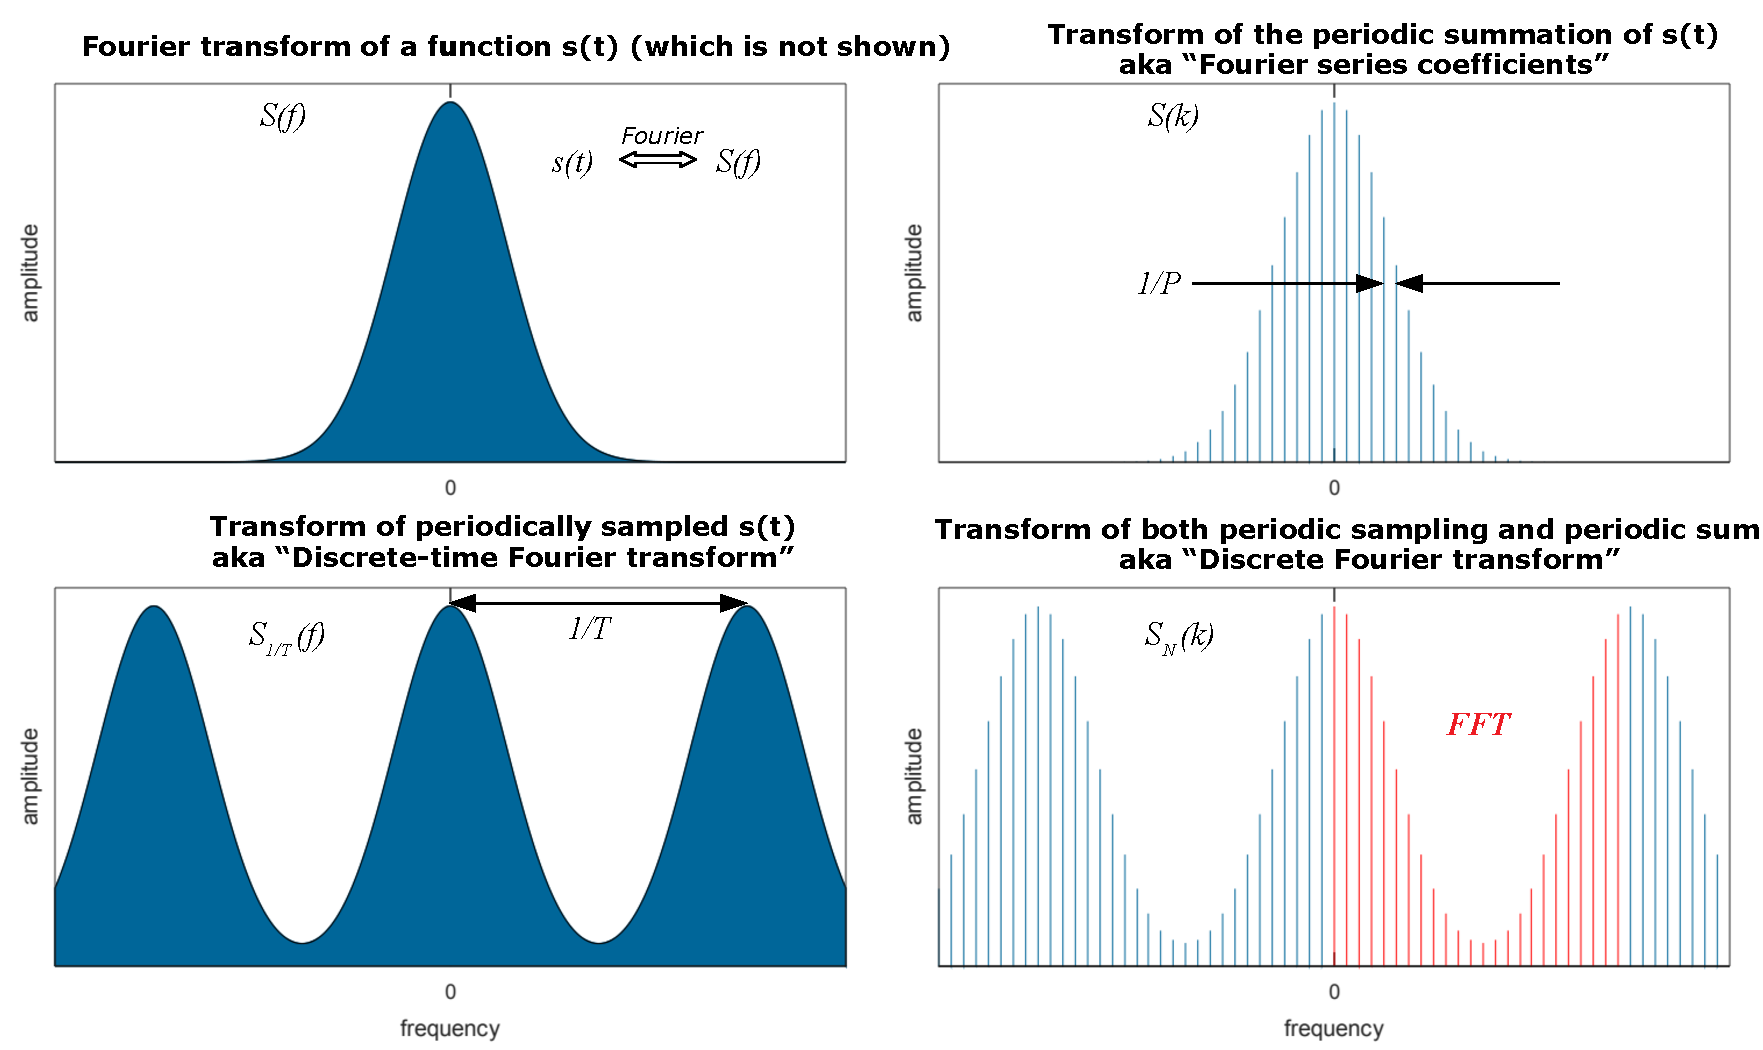
\includegraphics[width=5.5in]{fig/dft_sampling.pdf}
\end{center}
\caption{\label{fig:dft_sampling}Overview of sampling and periodicity
  effects in frequency space. Given the Fourier transform of a
  function (top left), sampling it every T time may cause a change in
  the frequency space values according to the sampling theorem (bottom
  left). This is called aliasing, in the bottom left panel, the
  minimum value shown is different from the top left panel. If the
  function is periodic, the frequency space values reduced to discrete
  values as well (top right). DFT/FFT combines the two concepts
  (bottom right). Considering unit pixel size, the FFT space always
  goes to 1/2 frequency with a resolution of 1/N. Figure source:
  Wikipedia:Discrete Fourier transform}
\end{figure}
%
\subsection{Zero padding in FFT frequency space\label{sec:zeropadS}}
%
\par While in image space convolution operations can have their own
way of handling edges, in Fourier space, multiplication always
corresponds to the circular boundary conditions in image space.  If we
want to implement a convolution without circular boundary
conditions that we want to calculate in frequency space,
we need to pad the images by extra edge pixels to avoid the
reappearance of values from the opposite side.
As we saw in \Cref{sec:patterns}, numerical artifacts in the matching
kernels cannot be bounded well in image space, they fill the full area
independently of the padding size. Therefore we cannot practically perform
the kernel matching convolutions in image space.
%
\par In the previous section, we also saw that a zero-padding violates one
of the ZOGY assumptions: that frequencies are independent and log
likelihoods can be calculated from them by simple addition. Is this a
significant inaccuracy in the score image?
%
\par Let's assume for a moment that the image background is extended in a
sourceless way with white noise. In this case, all the assumptions of the
detection statistics derivation hold thus we get \Cref{eq:Shat}. This is a
usual convolution expression in image space and at any pixel its value
depends only from the half \(P_d\) size neighboring area. If \(P_d\)
significant values are located in about the same square size as the original
PSF size then the affected edge area also remains the same. If the PSF
contains edges, however, \(P_d\) can be significantly bigger in size. Zero
padding adds pixels to an image that, from a noise model perspective, all
have a noise variance of zero. By padding the input images with zeroes, the
pixel variance of the difference image and, in a smaller edge region, the
score image variance will decrease. It is unclear whether scaling the score
image \(S\) with its variance plane satisfactorily corrects for this
effect. Nevertheless, this correction term is listed as a suggested
rescaling of the score image in the ZOGY paper Section 3.3. Beside this
correctional approach, we propose the implementation of padding with the
model white noise instead of constant zeroes in the future.
%
\subsection{Sampling}
\par It can be shown that Gaussians with \(0.95 < \sigma\), are well
sampled in the sense that \(3\sigma\) of their Fourier
transform Gaussian fit up to the 1/2 frequency limit. For
\(5\sigma\) fit, this is \(1.59 < \sigma\).


% Include all the relevant bib files.
% https://lsst-texmf.lsst.io/lsstdoc.html#bibliographies
\section{References} \label{sec:bib}
\renewcommand{\refname}{} % Suppress default Bibliography section
\bibliography{local,lsst,lsst-dm,refs_ads,refs,books}

% Make sure lsst-texmf/bin/generateAcronyms.py is in your path
\section{Acronyms} \label{sec:acronyms}
\addtocounter{table}{-1}
\begin{longtable}{p{0.145\textwidth}p{0.8\textwidth}}\hline
\textbf{Acronym} & \textbf{Description}  \\\hline

1D & One-dimensional \\\hline
2D & Two-dimensional \\\hline
DM & Data Management \\\hline
DMTN & DM Technical Note \\\hline
FFT & Fast Fourier Transform \\\hline
LSST & Legacy Survey of Space and Time (formerly Large Synoptic Survey Telescope) \\\hline
PSF & Point Spread Function \\\hline
\end{longtable}

% If you want glossary uncomment below -- comment out the two lines above
%\printglossaries

\end{document}
